\section{Background and Motivation}
\label{sec:motivation}

%% UnsafeIterator is NOT a JAVA property!

\subsection{Finite State Properties}
\label{sec:motivation:fsp}

\begin{figure}[t]
\centering
  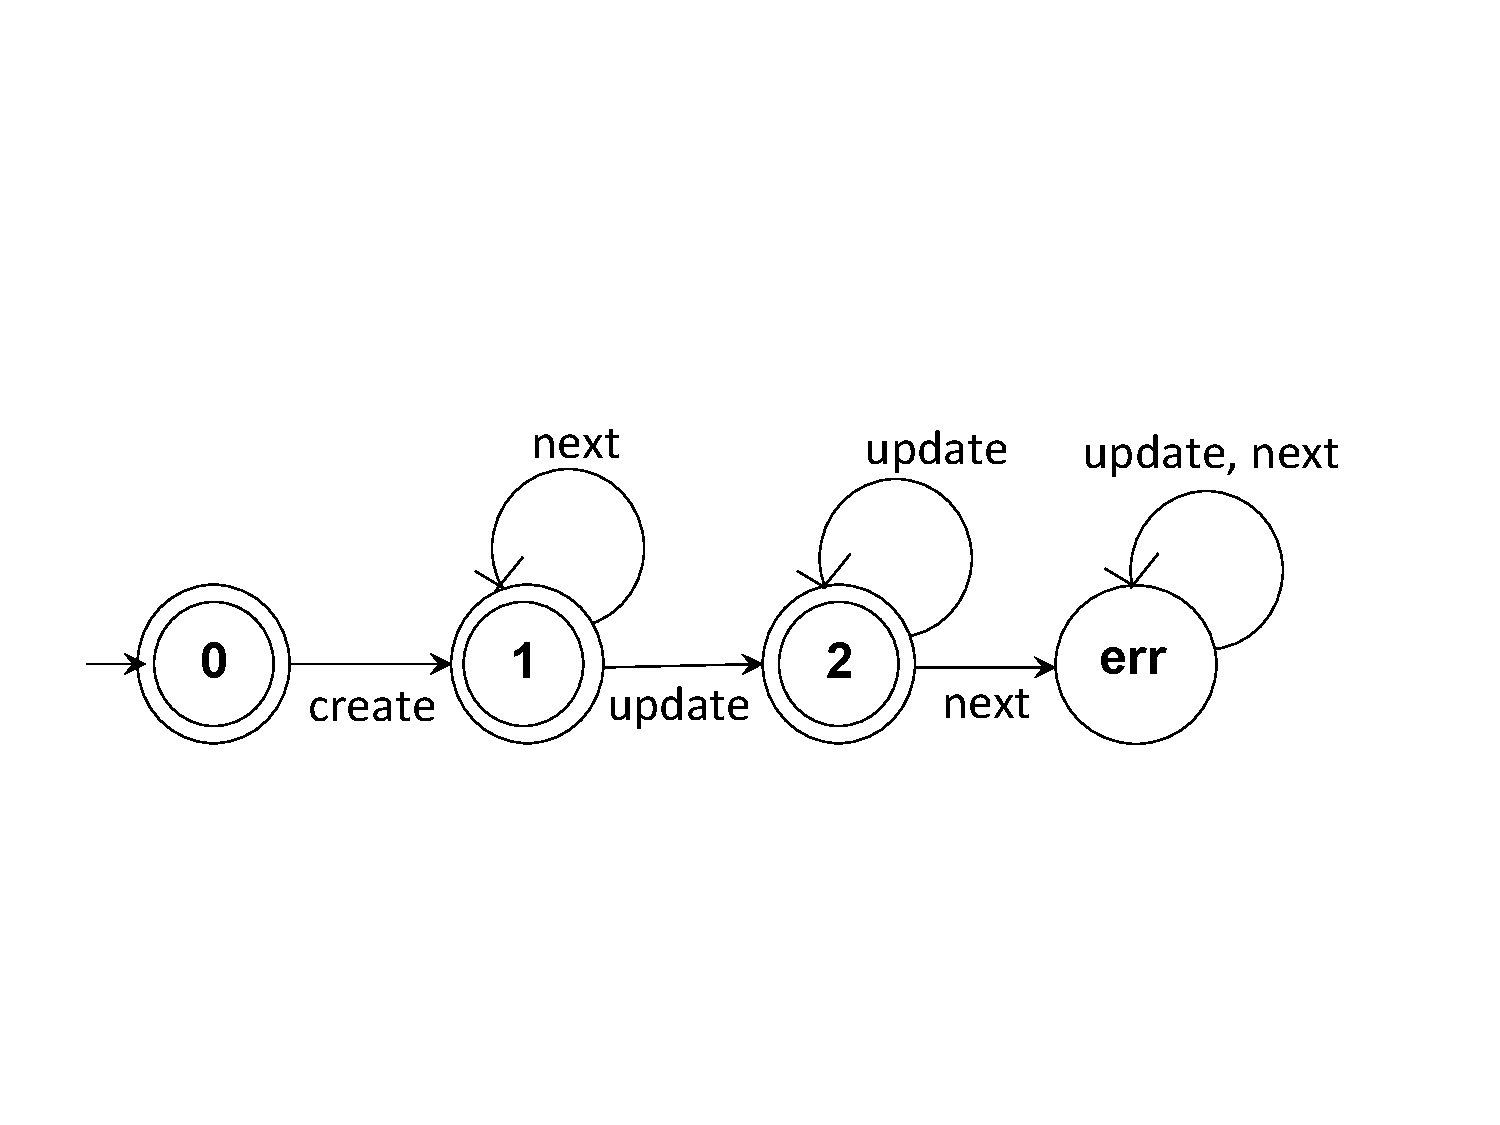
\includegraphics[scale=0.3, trim=0 5cm 0 6cm]{./images/unsafeiterator.pdf}
  \caption[UnsafeIterator Property FSA]{UnsafeIterator Property.}
  \label{fig:unsafeiteratorfsa}
\end{figure}

\begin{figure}[t]
\centering
  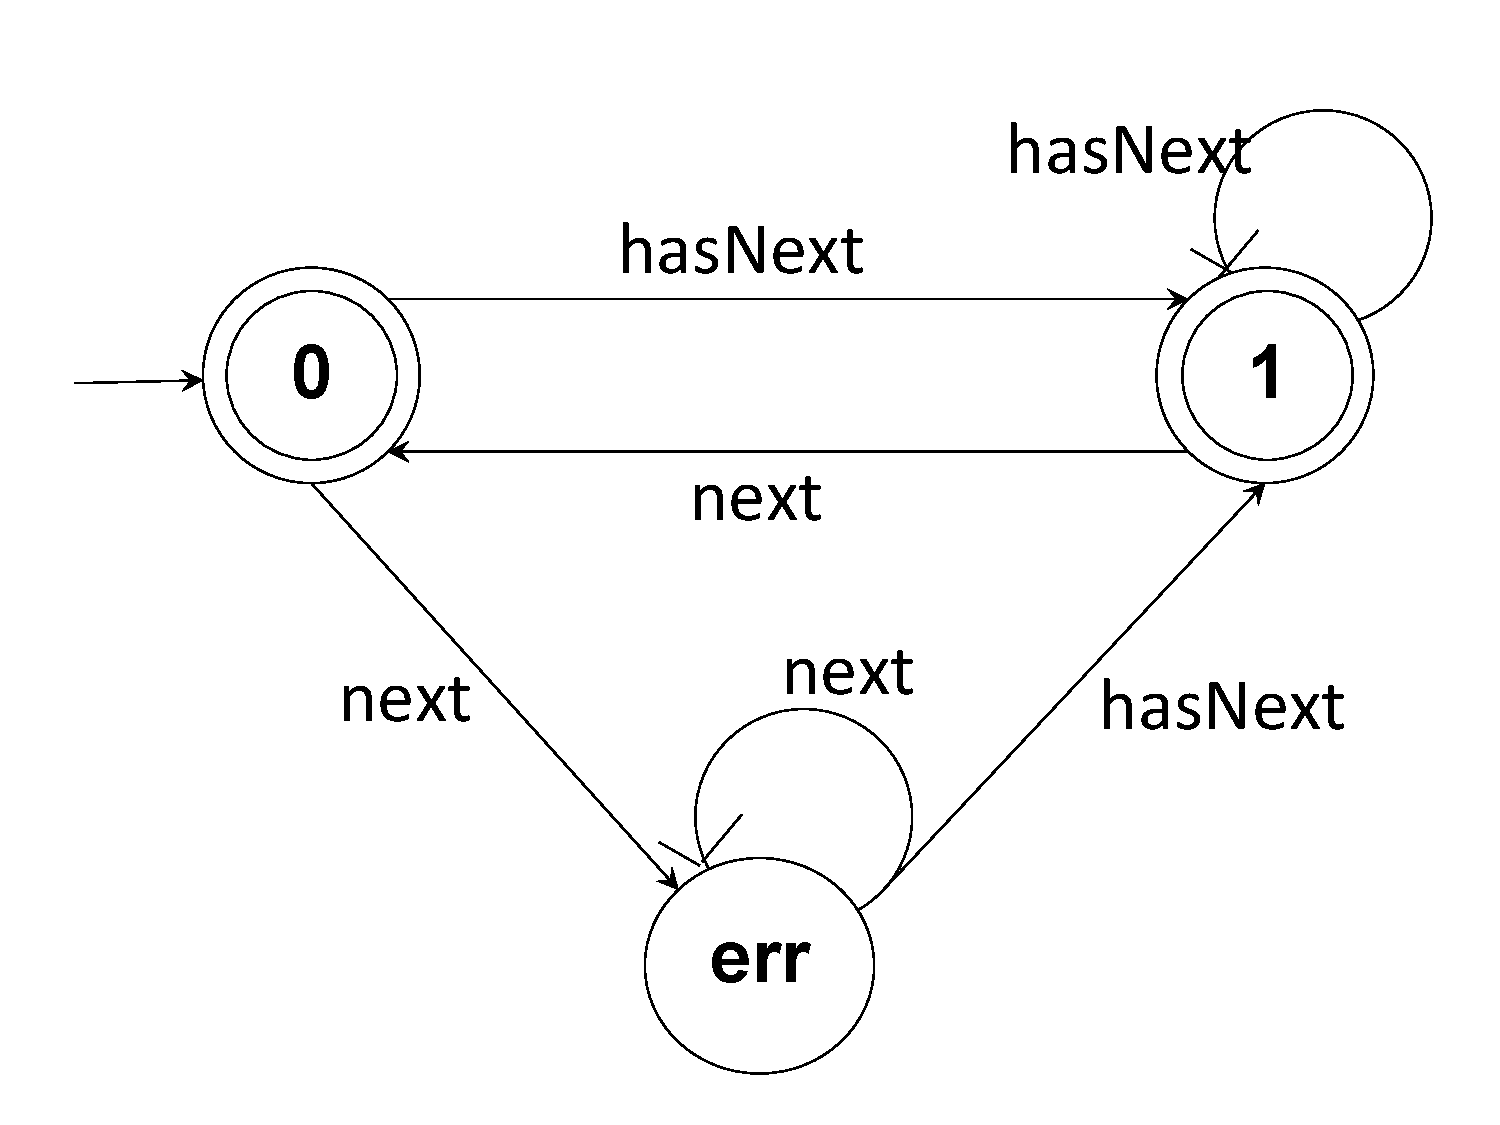
\includegraphics[trim=20cm 0cm 15cm 1cm, scale=0.2]{./images/HasNext.pdf}
  \caption[HasNext Property FSA]{HasNext Property.}
  \label{fig:hasnextfsa}
\end{figure}

Figure~\ref{fig:unsafeiteratorfsa} depicts a finite state automaton (FSA), 
which models iteration over a \code{Collection}, and codifies that a 
\code{Collection} must never be updated while it is being iterated over. The 
symbols \textit{create}, \textit{update}, and \textit{next} correspond to 
creating an \code{Iterator} from a \code{Collection}, modifying the 
\code{Collection}, and iterating over the said \code{Collection}, respectively. 
As shown in the figure, the symbol \textit{next} (observed following an 
\textit{update}) indicates iteration after a \code{Collection} update, and 
pushes the FSA to the \textit{error} state. Similarly, 
Figure~\ref{fig:hasnextfsa} encodes \code{Iterator} property \code{HasNext}, 
which states that \code{HasNext} must be invoked every time prior to invoking 
\textit{next} to ensure that the object exists before it is operated upon.

\subsection{Monitoring Systems}
\label{sec:motivation:monitor}

\code{Collection}s and \code{Iterator}s are commonly used objects, and also 
frequent sources of errors \cite{}. Thus, common monitoring systems, like 
\textsc{JavaMOP} typically instantiate a \textit{monitor} corresponding to every 
pair of \code{Collection} and \code{Iterator}, and use it to track the 
specified finite state properties upon occurrence of every event. For example, 
the monitoring system may create a new monitor for the \textit{creation} event, 
which corresponds to an invocation to the \code{Iterator()} method on the 
\code{Collection} interface, and returns an instance of the \code{Iterator}.
This newly created monitor is associated with both the \code{Collection} and 
the \code{Iterator} objects.

%% why is it a challenge
\myparagraph{Challenges} Efficient monitoring of finite state properties is 
thus usually a challenge due to:

\begin{table}[t]
\centering
\begin{tabular}{|c|c|c|c|c|}
\hline
\multirow{2}{*}{} & \multicolumn{2}{c|}{HasNext} & 
\multicolumn{2}{c|}{UnsafeIterator} \\
\cline{2-5} 
                  & monitors     & events        & monitors         & events    
 
      \\ \hline
avrora            & 0.8M      & 1.5M       & 0.9M         & 1.4M          \\ 
\hline
bloat             & 1.9M      & 162M    & 1.9M          & 82M         \\ \hline
pmd               & 8.6M      & 47M      & 1.9M          & 26M         \\ \hline
\end{tabular}
\caption{Number of monitors created and events generated for different programs 
and properties. \note{Get numbers for all benchmarks.}}
\end{table}
\label{table:numofmonitors}

\begin{table}[t]
\centering
\begin{tabular}{|c|c|c|c|}
\hline
%\multirow{2}{*}{} & \multicolumn{2}{c|}{HasNext} & 
% \multicolumn{2}{c|}{UnsafeIterator} \\ \cline{2-5}
 {} & Original & HasNext & UnsafeIterator\\
 \hline
avrora            & 0.1G      & 0.4G(300\%)       & 0.7G(600\%)           \\ 
\hline
bloat             & 0.5G      & 1.1G(120\%)    & 1.3G(160\%)              \\ 
\hline
pmd               & 0.5G      & 0.6G(20\%)     & 1.0G(100\%)             \\ 
\hline
\end{tabular}
\caption{Memory consumption for different programs and properties with and 
without monitoring. The figures in the parentheses are the percentage 
overheads. \note{Get numbers for all benchmarks.}}
\end{table}
\label{table:consumedmemory}

\begin{challenges}
 \item \textbf{High monitor count}: Typically, in practice, a \code{Collection} 
object may get iterated over several times before getting garbage collected. 
Coupled with the fact that both \code{Collection}s and \code{Iterator}s are 
frequently used objects in most programs, the number of monitors grows 
exponentially. Table~\ref{table:numofmonitors} lists the huge number of 
monitors observed when monitoring three commonly used \textsf{DaCapo} benchmarks 
for \code{HasNext} and \code{UnsafeIterator} properties using with JavaMOP 
v$2.3$. The huge number of monitors even for a relatively small number of 
monitored \code{Collection} and \code{Iterator} objects puts a significant 
burden on the system and the garbage collector. Furthermore, if the monitor 
objects are live, the garbage collector cannot even reclaim them.
 
 \item \textbf{High memory usage}: Table~\ref{table:consumedmemory} lists the 
memory consumption of the benchmarks with and without monitoring using 
\textsc{JavaMOP} v$2.3$. We observe that the large number of monitors results 
significantly large memory consumption, in contrast to the benchmarks' normal 
memory requirements, \ie\ without monitoring. Furthermore, in practice, 
programmers like to monitor programs for \textit{all} interesting properties 
collectively, and not individually. This collective monitoring of properties 
becomes extremely difficult, and often infeasible. Prior 
work~\cite{}\note{Purandare \etal} presents a technique to compact multiple 
monitors and track programs for several properties simultaneously. However, the 
resource footprint can still be significant and prohibitively high for 
resource-constrained systems, because compaction reaches its limit quickly when 
involving a finite state automata (FSA) product, which may itself grow 
exponentially.

 \item \textbf{High event tracking overhead}: In addition to the high overall 
resource consumption associated with monitors, the cost of handling individual 
events for tracking properties associated with multiple objects, such as 
\code{UnsafeIterator}, could potentially be prohibitive. This high cost is 
incurred since, theoretically, an unbounded number of monitors may get 
associated with the events (depending on the program and property interactions). 
As a result, the cost of tracking even a single event can become unpredictably 
large.
% 
In fact, we observed that over $1500$ monitors were associated with a single 
\code{Collection} object when monitoring for \code{UnsafeIterator} property 
for the \text{bloat} \textsf{DaCapo} benchmark. Since each of these monitors 
needs to be tracked when an event is handled by the corresponding receiver, 
monitoring all events, thus, becomes non-deterministic in terms of time. 
Furthermore, not being able to provide guaranteed bounds on the monitored 
execution significantly restricts the usage to non real-time systems or systems 
where performance guarantees are not essential. In any case, however, most 
systems suffer degraded performance with uncontrolled resource usage and 
execution overhead for monitoring systems.
 
 \item \textbf{Redundant monitors}: For the same set of \textsf{DaCapo} 
benchmarks and properties, we also observed that all $42$ errors reported while 
monitoring \textit{bloat} for property \texttt{HasNext}, and $333$ errors 
reported by \textit{pmd} can be partitioned into two distinct classes of errors 
that shared similar execution context, \ie\ the stack trace.
% 
% % we need not explain the optimization here.
% For this work, we associated an execution context with a method calling 
% sequence
% %a call stack and the program counter,
% and the data was collected  by considering limited execution context for 
% efficiency reasons. 
% 
These observations indicate that several monitors catch the same redundant 
errors, which clearly is not intelligent reporting to the developer. Ideally, 
the monitors must report only distinct errors, \ie\ only $3$ distinct errors 
for \textit{bloat}, and $2$ for \textit{pmd}. \note{This needs to be 
clarified --- 2 distinct classes, and 3 and 2 errors respectively.} Hence, we 
believe that sampling-based monitoring that leverage the program execution 
context would be significantly more effective and consume much less resources.
\end{challenges}

%We also made some fine-grain observations regarding the redundancy in the 
%behavior of monitors.  For the same DaCapo benchmarks and properties, 
%Table~\ref{table:joinpoints} presents the number of \textit{observable} 
%statements that generate monitoring events. Even though monitors are generated 
%in millions, observable statements are only a few. This indicates that there 
% is 
%a reason to believe that the \textit{programming contexts} under which these 
%statements are invoked are limited. 

In this work, we present a runtime verification approach that exploits 
redundancy in monitor behavior, and retains only those that show distinct 
behavior. As a result, put approach significantly improves upon memory 
efficiency and execution time determinism. 
% The approach has been described in detail in Section~\ref{sec:approach}.

\ignore{
Figure~\ref{fig:unsafeiteratorfsa} depicts a finite state automaton (FSA) that 
models a property \texttt{UnsafeIterator} which is defined by the API of Java 
standard library and is related to a \texttt{Collection} as well as an 
\texttt{Iterator} object. It specifies the rule that a collection should not be 
updated while it is being iterated. The symbols \textit{create}, 
\textit{update}, and \textit{next} correspond to creating an iterator from a 
collection, modifying a collection, and iterating over a collection 
respectively. Hence, as shown in the figure, the symbol \textit{next} observed 
after the symbol \textit{update} would indicate iteration after a collection 
update which pushes the FSA to the \textit{error} state. Monitoring systems 
typically instantiate a monitor corresponding to every such pair of a collection 
and an iterator and use it to track the FSA states depending on the sequence of 
operations or events encountered.

In practice, a collection object may get iterated several times in its life 
time. On the occurrence of a \textit{creation} event, that may correspond to the 
call to \textmd{Iterator()} method in the \textmd{Collection} interface that 
returns an iterator, a monitoring system may create a new monitor for tracking. 
The newly created monitor is associated with the collection object and also the 
iterator object. It is easy to see that since the collection and iterator are 
frequently used objects in many programs the number of monitors may grow 
quickly. This puts heavy burden on the system and the garbage collector. 
Moreover, if the monitor objects are live, garbage collector cannot reclaim 
them.

Similar issue arises with another iterator property \texttt{HasNext} depicted in 
Figure~\ref{fig:hasnextfsa}. It specifies that a call to the \textit{hasNext} 
method must be given before calling \textit{next} method to ensure that an object 
exists before it is used. Collections and iterators are not only commonly used 
objects, but often the sources of error \cite{}.
}

\ignore{
Monitoring finite state properties efficiently has been a challenge due to the 
large number of monitors that may get created and also due to the large number 
of monitors that may get associated with some events. 
Table~\ref{table:numofmonitors} shows the number of monitors we observed while 
monitoring some \textsf{DaCapo} benchmarks using JavaMOP 2.3 for 
\texttt{HasNext} and 
\texttt{UnsafeIterator} properties.
}

\ignore{
\begin{itemize}
\item {\bf HasNext}: Every call to method \texttt{next} associated with an 
iterator must be preceded by a call to method \texttt{hasNext}.
\item {\bf UnsafeIterator}: A collection should not be updated while it is being 
iterated.
\end{itemize}
}

\ignore{
Table~\ref{table:consumedmemory} presents the memory consumption of the 
benchmarks with and without monitoring when JavaMOP 2.3 was used for monitoring. 
It shows that the large number of monitors results in the consumption of 
significantly large amount of memory in comparison with the benchmarks' memory 
requirements. Moreover, in practice, programmers would like to monitor their 
programs for all of the interesting properties together, not separately. This 
only means that runtime monitoring would become extremely difficult or even 
infeasible when properties are monitored simultaneously. Purandare et al. 
present a technique that compacts several monitors into one and tracks programs 
for multiple properties simultaneously \cite{}. However, even though the compaction 
reduces the footprint of a monitored program to a certain extent, the footprint 
can still be significant and prohibitively high for 
resource-constrained systems. This is owing to the fact that the compaction 
reaches its limit quickly since 
it involves taking a finite state automata (FSA) product which may grow 
exponentially.
}

\ignore{
In addition to the overall high overheads, for the properties associated with 
multiple objects, such as \texttt{UnsafeIterator} the cost of handling 
individual events can also be very high. This  happens since theoretically unbounded number of 
monitors may get associated with the events depending on the program and 
property interactions. As a result, the cost of tracking one single event can become 
unpredictably large. In fact, it was observed while monitoring for 
\texttt{UnsafeIterator} property for the \textsf{DaCapo} benchmark 
\textit{bloat} that as many as 1548 monitors had got associated with a single 
\textsf{Collection} object. Each of these monitors needs to be tracked when an 
event is seen by the corresponding receiver object. As a result, monitoring 
actions become nondeterministic in terms of time. Not being able to provide
bounds to the monitoring execution can 
restrict the usage of monitoring to nonreal-time systems or systems where 
performance guarantees are not essential. 
However, most systems in practice would suffer due to degraded performance if 
the memory overheads and execution times of monitoring cannot be controlled.

%We also made some fine-grain observations regarding the redundancy in the 
%behavior of monitors.  For the same DaCapo benchmarks and properties, 
%Table~\ref{table:joinpoints} presents the number of \textit{observable} 
%statements that generate monitoring events. Even though monitors are generated 
%in millions, observable statements are only a few. This indicates that there is 
%a reason to believe that the \textit{programming contexts} under which these 
%statements are invoked are limited. 

For the same \textsf{DaCapo} benchmarks and properties, we made some fine-grain 
observations regarding the redundancy in the behavior of monitors. We observed 
that the 42 errors reported while monitoring \textit{bloat}  for property 
\texttt{HasNext} could be partitioned into two classes of errors such that all 
errors in a class had a similar \textit{execution context}. Similarly, we could 
divide 333 errors reported by \textit{pmd} into two classes. For this work, we 
associated an execution context with a method calling sequence
%a call stack and the program counter,
and the data was collected  by considering limited execution context for efficiency 
reasons. These observations indicate that many monitors catch redundant errors, 
which are not so useful to developers. Ideally, the reporting should only be 
performed for distinct errors which means catching only thee distinct errors for 
\textit{bloat} and two for \textit{pmd} would suffice. Hence, we believe that 
monitoring performed by sampling objects based on the program execution context 
could be effective and would require less resources. 

In this work, we present a runtime verification approach that tries to exploit 
the redundancy in the monitor behavior and retain only the ones that show 
distinct behavior. As a result, it improves on memory efficiency as well as execution time 
determinism. The approach has been described in detail in 
Section~\ref{sec:approach}.
}

\ignore{
Some very particular typestate properties are typically desired to be satisfied 
by all programs. The traditional runtime-verification approach has been 
developed over the past decade to analyze large complex applications because of 
several desirable properties. For instance, because the monitor specifications 
can be very expressive as runtime monitoring reason about concrete program 
events and runtime objects, and thus avoid false warnings. Also, when a runtime 
monitor detects a property violation, it can respond to this violation in many 
different ways, which can be any code from information logging to runtime 
recovery. The programmer has the guarantee that the monitor will detect a 
violation if it exists.\\
\begin{table}[h]
\centering
\begin{tabular}{|c|c|c|c|c|}
\hline
\multirow{2}{*}{} & \multicolumn{2}{c|}{HasNext} & 
\multicolumn{2}{c|}{UnsafeIterator} \\ \cline{2-5} 
                  & monitors     & events        & monitors         & events     
      \\ \hline
avrora            & 805500       & 1507792       & 909011           & 1365801    
      \\ \hline
bloat             & 1906736      & 162227791     & 1876472          & 82032703   
      \\ \hline
pmd               & 8576900      & 47231567      & 1949816          & 25958426   
      \\ \hline
\end{tabular}
\caption{Number of monitors created and events generated for different programs 
and properties}
\end{table}

On the other hand, existing tools for runtime monitoring usually incur an 
unacceptable overhead. Large number of monitors created during runtime and the 
events generated by the program execution are responsible for the overhead. In 
our experiments, for Dacapo benchmarks bloat and pmd benchmarks create nearly 
the same number of monitors, in excess of a few million, for property 
UnSafeIterator for JavaMOP[4]. Table 2.1 shows the large number of monitors 
created and the events generated during runtime of several programs from Dacapo 
Benchmark suite.
\\\\With the motivation that there is a large redundancy among monitors in terms 
of their behavior which results in many monitors detecting same errors, we 
investigate the trade-off between the runtime overhead and the error reporting. 
We propose a runtime verification framework that is memory efficient and time 
deterministic and can be used for real time embedded systems. The framework has 
the following characteristics:
\begin{itemize}
	\item \textit{Object based sampling}: we introduce object based sampling 
to collect sampled objects on which monitoring will be performed. The heuristics 
applied for sampling are related to the program execution context. We achieve it 
by obtaining the call-stack contents.  obtain the method calls invoked on the 
current runtime object under analysis and compare whether the trace of method 
calls of that object has been previously seen during runtime. 
	\item \textit{Deterministic monitoring}: For multi-object properties 
such as UnsafeIterator property, an event such as update can get associated with 
several monitors. This number can grow uncontrollably and can be as large as 
1548 for an event [9]. It becomes difficult to keep track of every monitor for 
that event. Hence, the whole operation of handling events may become non 
deterministic as far as timing requirements are concerned. We consider a 
monitoring behaviour to be deterministic as we can calculate the time taken to 
perform monitoring by the cost model presented. We are controlling the monitors 
associated with each event to make tracking deterministic.
	\item \textit{Limited number of monitors to make memory efficient}: we 
consider to limit the total number of monitors generated while runtime 
verification and at the same time maintaining sufficient accuracy for detecting 
property violations.
\end{itemize}
Runtime Monitoring is complete but fundamentally unsound since it cannot see 
anything beyond the current execution. In our approach, we sacrifice on the 
soundness to achieve memory efficiency and determinism in terms of time.
}